\documentclass[10pt,letterpaper,twocolumn]{article}

\usepackage[top=2.1cm,left=2.0cm,right=2.0cm,footskip=2.0cm]{geometry}
\usepackage[utf8]{inputenc}     % for Unicode
\usepackage{cite}               % citation
\usepackage[dvipdfmx]{hyperref} % links
\usepackage{caption}            % caption
\usepackage{microtype}          % improves typesetting in LaTeX
\usepackage{graphicx}

% \usepackage{color}
% ex.) \textcolor{color}{text}

\begin{document}

\twocolumn[
    \begin{flushleft}
        {\Large
        \textbf\newline{An Extention of R-Tree for Periodic Boundary Conditions}
        }
        \newline
        \\
        Toru Niina \textsuperscript{1}
        \\
        \bigskip
        \bf{1.} Department of Biophysics, Graduate School of Science,
                Kyoto University, Kyoto 606-8502, Japan
        \\
        \bigskip
        * niina@theory.biophys.kyoto-u.ac.jp
    \end{flushleft}

    \section*{Abstract}
    Spatial searching is an important operation for physical, chemical, and
    biological simulations which run mostly on periodic boundary conditions.
    An R-Tree is a widely used data structure to manage spatial data objects and
    it is capable of processing a spatial searching query in an efficient way.
    Currently, several methods to handle an R-Tree on periodic boundary
    conditions have been proposed. Those methods keep the underlying R-Tree
    structure intact but modify queries or entire system. In this paper, I
    propose a new method to make the spatial structure of R-Tree itself along
    the periodic boundary conditions introducing a set of operations for
    rectangles on the condition. It will remove the requirements for extensional
    queries or copies of objects.
    \bigskip
]

\section*{Introduction} % the '*' after section prevents numbering
Lorem ipsum dolor sit amet, consectetur adipiscing elit. Aliquam bibendum
finibus diam, gravida sagittis lorem gravida vitae. Interdum et malesuada fames
ac ante ipsum primis in faucibus. Nulla in diam tristique ante posuere
tristique. Donec interdum purus sit amet nisl accumsan consectetur. Fusce
aliquet libero mi, quis ornare dolor congue ullamcorper. Nulla nulla urna,
molestie in urna sed, lacinia volutpat eros. Ut mi libero, elementum scelerisque
ipsum vel, hendrerit fermentum turpis. Aliquam sit amet leo sodales, egestas
augue id, fermentum nulla. Aenean vel cursus ante, et pellentesque eros. Nulla
ac neque nec justo posuere commodo sit amet sit amet justo. Aliquam tincidunt
tempor ex nec tincidunt. In ullamcorper vehicula lobortis.

\begin{figure}[hbt]
    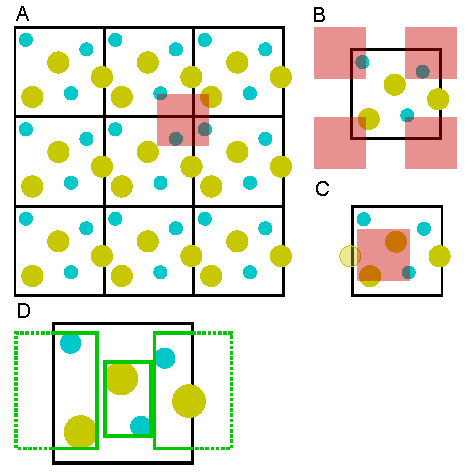
\includegraphics[width=6.5cm, bb=0 0 567 567]{fig1.eps}
    \caption{this is an example figure for the R-Tree structure}
    \label{fig1}
\end{figure}

\section*{Methods}

\paragraph{Paragraph.}
Lorem ipsum dolor sit amet, consectetur adipiscing elit. Aliquam bibendum
finibus diam, gravida sagittis lorem gravida vitae. Interdum et malesuada fames
ac ante ipsum primis in faucibus. Nulla in diam tristique ante posuere
tristique. Donec interdum purus sit amet nisl accumsan consectetur. Fusce
aliquet libero mi, quis ornare dolor congue ullamcorper. Nulla nulla urna,
molestie in urna sed, lacinia volutpat eros. Ut mi libero, elementum scelerisque
ipsum vel, hendrerit fermentum turpis. Aliquam sit amet leo sodales, egestas
augue id, fermentum nulla. Aenean vel cursus ante, et pellentesque eros. Nulla
ac neque nec justo posuere commodo sit amet sit amet justo. Aliquam tincidunt
tempor ex nec tincidunt. In ullamcorper vehicula lobortis.

\subsection*{Formulas.}
Lorem ipsum dolor sit amet, consectetur adipiscing elit. Aliquam bibendum
finibus diam, gravida sagittis lorem gravida vitae. Interdum et malesuada fames
ac ante ipsum primis in faucibus. Nulla in diam tristique ante posuere
tristique. Donec interdum purus sit amet nisl accumsan consectetur. Fusce
aliquet libero mi, quis ornare dolor congue ullamcorper. Nulla nulla urna,
molestie in urna sed, lacinia volutpat eros. Ut mi libero, elementum scelerisque
ipsum vel, hendrerit fermentum turpis. Aliquam sit amet leo sodales, egestas
augue id, fermentum nulla. Aenean vel cursus ante, et pellentesque eros. Nulla
ac neque nec justo posuere commodo sit amet sit amet justo. Aliquam tincidunt
tempor ex nec tincidunt. In ullamcorper vehicula lobortis.
% \begin{center}
\begin{eqnarray}
    f(x) &=& \mathrm{e}^x \nonumber\\
    g(x) &=& \log(x)      \nonumber
\end{eqnarray}
% \end{center}

\section*{Results}
\subsection*{subsection 1}
Lorem ipsum dolor sit amet, consectetur adipiscing elit. Aliquam bibendum
finibus diam, gravida sagittis lorem gravida vitae. Interdum et malesuada fames
ac ante ipsum primis in faucibus. Nulla in diam tristique ante posuere
tristique. Donec interdum purus sit amet nisl accumsan consectetur. Fusce
aliquet libero mi, quis ornare dolor congue ullamcorper. Nulla nulla urna,
molestie in urna sed, lacinia volutpat eros. Ut mi libero, elementum scelerisque
ipsum vel, hendrerit fermentum turpis. Aliquam sit amet leo sodales, egestas
augue id, fermentum nulla. Aenean vel cursus ante, et pellentesque eros. Nulla
ac neque nec justo posuere commodo sit amet sit amet justo. Aliquam tincidunt
tempor ex nec tincidunt. In ullamcorper vehicula lobortis.

\subsection*{subsection 2}
Lorem ipsum dolor sit amet, consectetur adipiscing elit. Aliquam bibendum
finibus diam, gravida sagittis lorem gravida vitae. Interdum et malesuada fames
ac ante ipsum primis in faucibus. Nulla in diam tristique ante posuere
tristique. Donec interdum purus sit amet nisl accumsan consectetur. Fusce
aliquet libero mi, quis ornare dolor congue ullamcorper. Nulla nulla urna,
molestie in urna sed, lacinia volutpat eros. Ut mi libero, elementum scelerisque
ipsum vel, hendrerit fermentum turpis. Aliquam sit amet leo sodales, egestas
augue id, fermentum nulla. Aenean vel cursus ante, et pellentesque eros. Nulla
ac neque nec justo posuere commodo sit amet sit amet justo. Aliquam tincidunt
tempor ex nec tincidunt. In ullamcorper vehicula lobortis.

\section*{Discussion}

Lorem ipsum dolor sit amet, consectetur adipiscing elit. Aliquam bibendum
finibus diam, gravida sagittis lorem gravida vitae. Interdum et malesuada fames
ac ante ipsum primis in faucibus. Nulla in diam tristique ante posuere
tristique. Donec interdum purus sit amet nisl accumsan consectetur. Fusce
aliquet libero mi, quis ornare dolor congue ullamcorper. Nulla nulla urna,
molestie in urna sed, lacinia volutpat eros. Ut mi libero, elementum scelerisque
ipsum vel, hendrerit fermentum turpis. Aliquam sit amet leo sodales, egestas
augue id, fermentum nulla. Aenean vel cursus ante, et pellentesque eros. Nulla
ac neque nec justo posuere commodo sit amet sit amet justo. Aliquam tincidunt
tempor ex nec tincidunt. In ullamcorper vehicula lobortis.

\bibliography{library}
\bibliographystyle{abbrv}

\end{document}
